\section{Baseline MLP}

\begin{itemize}
    \item Final training accuracy: \textbf{99.79\%}
    \item Final validation accuracy: \textbf{97.74\%}
    \item Number of parameters: \textbf{535,818}
\end{itemize}

\begin{figure}[h]
    \centering
    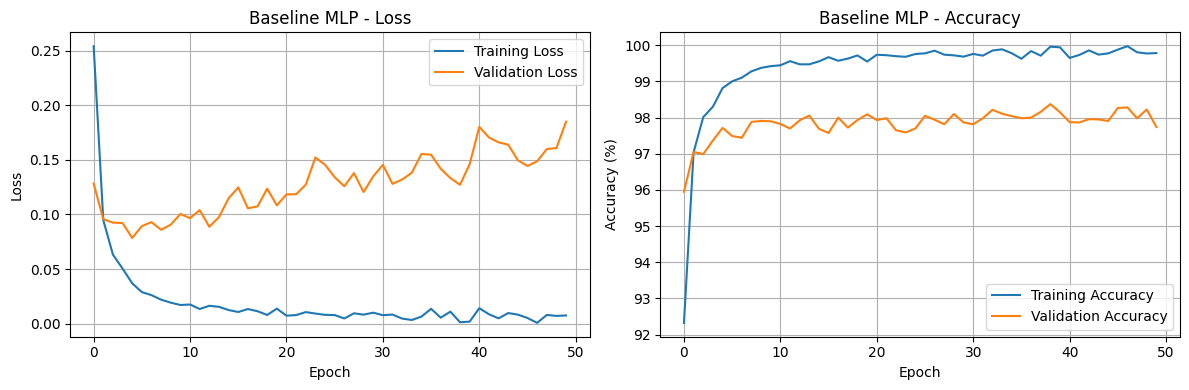
\includegraphics[width=0.7\linewidth]{section1/baselineMLP.png}
    \caption{Training and validation curves for Baseline MLP}
    \label{fig:baseline}
\end{figure}

\subsection{Question 1.1: Is the model overfitting?}
Yes, the model is overfitting. The training loss approaches zero while validation loss increases after epoch 10, with a 2.05\% gap between training (99.79\%) and validation (97.74\%) accuracy. This indicates the model memorizes training data rather than generalizing.

\subsection{Question 1.2: When does overfitting begin?}
Overfitting begins around epoch 10-15, when validation loss stops improving and starts increasing while training loss continues decreasing.